\section{Comparison to \texorpdfstring{\citet{altabaa2024abstractors}}{Altabaa et al. (2024)}: Abstractors and Relational Cross-Attention}\label{sec:appdx_abstrator}

A closely related work is \citet{altabaa2024abstractors}, which proposes a Transformer-based module called the ``Abstractor'' with relational inductive biases. The core operation in the Abstractor is a variant of attention dubbed ``relational cross-attention'' (RCA). In this section, we will discuss the relation between the Dual Attention Transformer and the Abstractor.

\subsection{Comparison between RA (this work) and RCA \texorpdfstring{\citep{altabaa2024abstractors}}{(Altabaa et al., 2024)}}

\citet{altabaa2024abstractors} propose a variant of attention called relational cross-attention which shares some characteristics with our proposal of what we're calling ``relational attention'' in this work. In this discussion, we will use the acronyms RCA and RA, respectively to distinguish between the two.

RCA processes a sequence of objects $\x = (x_1, \ldots, x_n)$ and produces a sequence of objects $\x' = (x_1', \ldots, x_n')$ via the following operation
\begin{align*}
    \x' &\gets \sigma_{\mathrm{rel}}\paren{\phi_q(\x) {\phi_k(\x)}^\intercal} \s, \\
    \s &= \SymbolRetriever(\x)
\end{align*}
where $\phi_q, \phi_k$ are query and key transformations, and the symbols $\s$ take the same role as in this work. $\sigma_{\mathrm{rel}}$ is referred to as a ``relation activation''. It may be either softmax or an element-wise activation (e.g., tanh, sigmoid, or linear). For the purposes of this discussion, let us consider $\sigma_{\mathrm{rel}} = \Softmax$, which was used in the majority of the experiments in~\citep{altabaa2024abstractors}.

To facilitate the discussion, let us write RA and RCA side-by-side using a common notation.

\aafatal{TODO --- change to row-vector format? i.e., $r_{ij} W_r$ instead of $W_r r_{ij}$, etc. match main body of paper. }
\begin{align*}
&\text{RA (this work)}    & &\text{RCA \citep{altabaa2024abstractors}}\\
(x_1', \ldots, x_n') &\gets \RA(\x; \Slib), & (x_1', \ldots, x_n') &\gets \RCA(\x; \Slib)\\
x_i' &= \sum_{j=1}^{n} \alpha_{ij} \, \bigparen{W_r \, r(x_i, x_j) + W_s \, s_j}, & x_i' &= \sum_{j=1}^{n} \alpha_{ij} \, s_j,\\
\bm{\alpha} &= \Softmax\bigparen{\phi_q(\x) {\phi_k(\x)}^\intercal}, & \bm{\alpha} &= \Softmax\bigparen{\phi_q(\x) {\phi_k(\x)}^\intercal},\\
r(x, y) &= \bigparen{\iprod{\phi_{q,\ell}^{\rel}(x)}{\phi_{k,\ell}^{\rel}(y)}}_{\ell \in [d_r]}, & \\
(s_1, \ldots, s_n) &= \SymbolRetriever(\x;\,\Slib) & (s_1, \ldots, s_n) &= \SymbolRetriever(\x;\,\Slib)
\end{align*}

% an unsuccessful attempt to format this with a table
% \begin{tabular}{p{0.45\textwidth}|p{0.45\textwidth}}
%     % RA (this work) & RCA \citep{altabaa2024abstractors} \\\midrule
%     {\begin{align*}
%         &\text{RA (this work)} \\
%         (x_1', \ldots, x_n') &\gets \RA(\x; \Slib), \\
%         x_i' &= \sum_{j=1}^{n} \alpha_{ij} \bigparen{W_r \, r(x_i, x_j) + W_s \, s_j}, \\
%         \bm{\alpha} &= \Softmax\bigparen{\phi_q(\x) {\phi_k(\x)}^\intercal}, \\
%         r(x, y) &= \bigparen{\iprod{\phi_{q,\ell}^{\rel}(x)}{\phi_{k,\ell}^{\rel}(y)}}_{\ell \in [d_r]}, \\
%         (s_1, \ldots, s_n) &= \SymbolRetriever(\x;\,\Slib)
%     \end{align*}} &  
%     {\begin{align*}
%         & \text{RCA \citep{altabaa2024abstractors}} \\
%         (x_1', \ldots, x_n') &\gets \RCA(\x; \Slib), \\
%         x_i' &= \sum_{j=1}^{n} \alpha_{ij} W_s \, s_j, \\
%         \bm{\alpha} &= \Softmax\bigparen{\phi_q(\x) {\phi_k(\x)}^\intercal}, \\
%         &\hphantom{r(x, y) = \bigparen{\iprod{\phi_{q,\ell}^{\rel}(x)}{\phi_{k,\ell}^{\rel}(y)}}_{\ell \in [d_r]},} \\
%         (s_1, \ldots, s_n) &= \SymbolRetriever(\x;\,\Slib)
%     \end{align*}}
%     \\
% \end{tabular}

RCA can be understood as self-attention, but the values are replaced with symbols (i.e., $\Attn(Q \gets \x,\, K \gets \x,\, V \gets \s)$). By viewing the attention scores $\alpha_{ij}$ as relations, this has the effect of producing a relation-centric representation. The rationale is that in standard self-attention, the attention scores form a type of relation, but these relations are only used in an intermediate processing step in an information-retrieval operation. The relations encoded in the attention scores are entangled with the object-level features, which have much greater variability. This thinking also motivates the design of RA in the present work.

RCA can be understood as computing a pairwise relation $\iiprod{\phiqattn(x_i)}{\phikattn(x_j)}$ between $x_i$ and each $x_j$ in the context, and retrieving the symbol $s_j$ associated with the object $x_j$ with which the relation is strongest. That is, RCA treats the relations and the attention scores as the same thing. By contrast, the attention operation and computation of relations are disentangled in RA. The attention component is modeled by one set of query/key maps $\phiqattn, \phikattn$ and the relation component is modeled by another set of query/key maps $(\phiqrell{\ell}, \phikrell{\ell})_{\ell \in [d_r]}$.

The intuitive reason for this choice is that, for many tasks, the optimal ``selection criterion'' will be different from the task-relevant relation. For example, in a language modeling task, you may want to attend to objects on the basis of proximity and/or syntax while being interested in a relation based on semantics. Similarly, in a vision task, you may want to attend to objects on the basis of proximity, while computing a relation across a certain visual attribute.

In RA, the symbols maintain the role of identifying the sender. But instead of being the whole message, they are attached to a relation.

\subsection{Comparison between \textit{DAT} and the Abstractor}

We now briefly discuss the differences in the resulting architectures.~\citet{altabaa2024abstractors} propose an encoder-like module called the Abstractor which consists of essentially replacing self-attention in an Encoder with relational cross-attention. That is, it consists of iteratively performing RCA followed by an MLP. The paper proposes several ways to incorporate this into the broader Transformer architecture. For example, some of the experiments use a $\texttt{Encoder} \to \texttt{Abstractor} \to \texttt{Decoder}$ architecture to perform a sequence-to-sequence task. Here, the output of a standard Transformer is fed into an Abstractor, and the Decoder cross-attends to the output of the Abstractor. In another sequence-to-sequence experiment, \citet{altabaa2024abstractors} use an architecture where the Decoder cross-attends to both the Encoder and the Abstractor, making use of both sensory and relational information. In particular, the standard encoder and decoder blocks are the same (focusing on sensory information), but an additional module is inserted in between with a relational inductive bias.

By contrast, our approach in this paper is to propose novel encoder and decoder architectures imbued with two distinct types of attention heads, one with an inductive bias for sensory information and the other with an inductive bias for relational information. This has several potential advantages. The first is versatility and generality. The Abstractor architectures that were explored in~\citep{altabaa2024abstractors} only explicitly support sequence-to-sequence or discriminative tasks. For example, they do not support autoregressive models like modern decoder-only language models (e.g., of the form we experiment with in~\Cref{ssec:tiny_stories}). Moreover, even in sequence-to-sequence tasks, Abstractor architectures only support relational processing over the input sequence, but they do not support relational processing over the target sequence (since the decoder does not have RCA). Another potential advantage of \textit{DAT} is simplicity. The Abstractor paper proposes several architectures and configurations for the Encoder/Abstractor/Decoder modules, introducing several hyperparameters that are not trivial to choose. Moreover, it is unclear how to interpret this kind of architecture as the number of layers increases, and the original paper does not experiment with scaling up the number of layers. The final potential advantage is increased expressivity. In \textit{DAT}, the two types of attention heads exist side by side in each layer. This allows relational attention heads to attend to the output of the self-attention heads at the previous layer, and vice-versa. This yields broader representational capacity, and potentially more interesting behavior as we scale the number of layers.

\subsection{How would RCA perform in an \textit{DAT}-style dual head-type architecture?}

One question one might ask is: how would an \textit{DAT}-style dual head-type architecture perform if we used \citet{altabaa2024abstractors}'s RCA instead of the RA head-type proposed in this work? We carried out a few ablation experiments to answer this question.

\Cref{fig:relgames_ratype_ablation} compares learning curves on the relational games benchmark between standard \textit{DAT} (with RA-heads) and a version of \textit{DAT} with \citet{altabaa2024abstractors}'s RCA heads. We find that the two models perform similarly, with most differences small enough to be within the margin of error. This figure depicts the configuration with asymmetric RA and positional symbols.

\Cref{fig:tinystories_ratype_ablation} depicts the validation loss curves on the Tiny Stories language modeling task, comparing standard \textit{DAT} against a version with RCA heads. Here, we find that our relational attention heads yield better-performing models, with the RCA-head variant of \textit{DAT} performing no better than a standard Transformer with a matching total number of heads.

\begin{figure}[ht]
    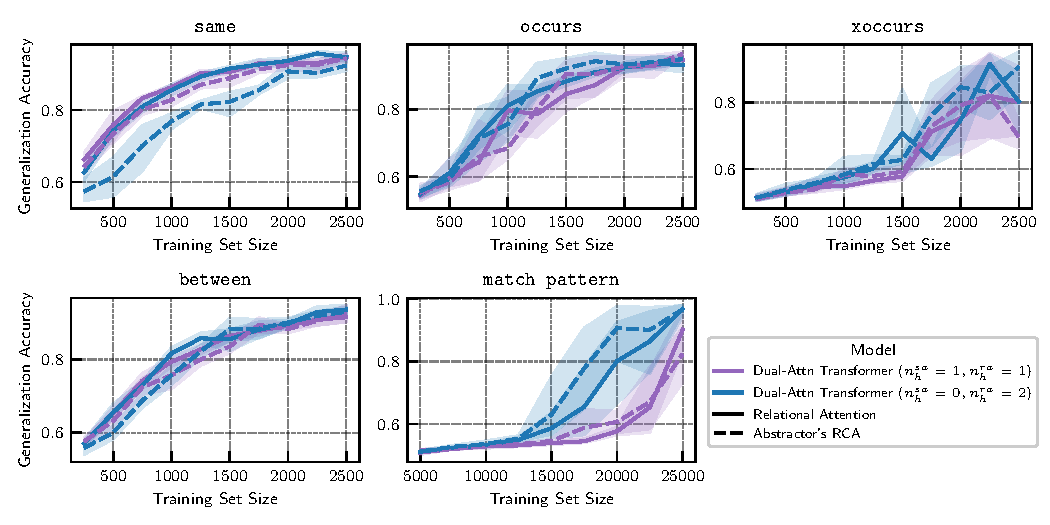
\includegraphics[width=\textwidth]{figs/experiments/relgames/relgames_learning_curves_rcatype_ablation.pdf}
    \caption{Learning curves for \textit{DAT} with RA compared with \textit{DAT} with RCA on the relational games benchmark. The performance is similar, with most differences within the margin of error.}\label{fig:relgames_ratype_ablation}
\end{figure}

\begin{figure}[ht]
    \centering
    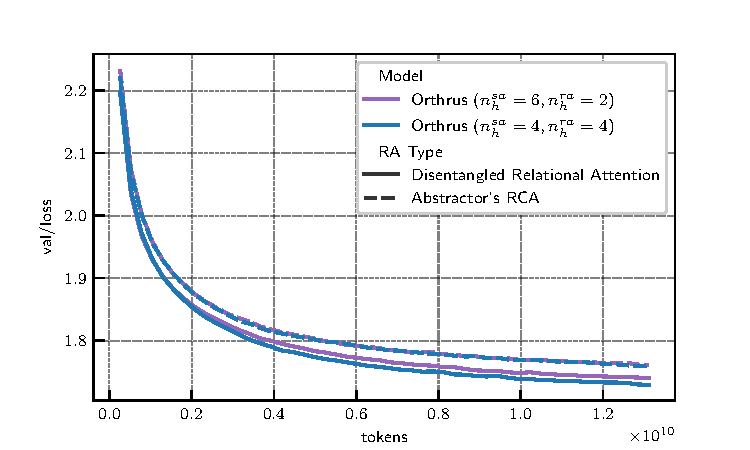
\includegraphics[width=0.5\textwidth]{figs/experiments/tiny_stories/d64L4_ra_type_ablation_symattn_asymra.pdf}
    \caption{Ablation of relational attention type. The solid line depicts the form of relational attention proposed in this work. The dotted line depicts RCA as proposed by \citet{altabaa2024abstractors}. We find that our relational attention mechanism performs better, whereas RCA performs no better than a Transformer.}\label{fig:tinystories_ratype_ablation}
\end{figure}